\documentclass[10pt,a4paper]{article}
\usepackage[margin=1.8cm]{geometry}
\usepackage{graphicx}
\usepackage{booktabs}
\usepackage{amsmath}
\usepackage{enumitem}
\usepackage[font=small,labelfont=bf]{caption}
\usepackage[colorlinks=true,urlcolor=blue,linkcolor=black,citecolor=black]{hyperref}
\graphicspath{{../results/figures/}{../results/report_assets/}}
\setlist{nosep,leftmargin=1.2em}
\setlength{\parskip}{3pt}
\setlength{\parindent}{0pt}
\emergencystretch=3em

\title{\vspace{-1.2cm}\textbf{Homework 2: Image Classification with Transfer Learning}\\[2pt]
\large Computer Vision, Fall 2026 -- University of Verona}
\author{Nuras Assylbekov (matricola VR565535)}
\date{}

\begin{document}
\maketitle
\vspace{-0.8cm}
\noindent\textbf{Repository (code, split files, metrics, checkpoints):}\\
\url{https://github.com/NurasAbi/cv-hw2-image-classification}

\section{Data}
I use the Oxford-IIIT Pet dataset~\cite{parkhi2012}: 7{,}349 images of 37 breeds (25 dog and 12 cat breeds), roughly 200 images per breed.
The target is the \emph{breed} (37 classes), not cat versus dog. The dataset is released by its authors under
\textbf{Creative Commons Attribution-ShareAlike 4.0}; the copyright of the images remains with the original owners.
It is not stored in the repository: the scripts download it with \texttt{OxfordIIITPet(download=True)} of TorchVision
(from \url{https://www.robots.ox.ac.uk/~vgg/data/pets/}).

\textbf{Splits.} The official \texttt{trainval} partition (3{,}680 images) is split 80/20 \emph{stratified by breed}
(scikit-learn \texttt{train\_test\_split}, \texttt{random\_state=42}) into
\textbf{2{,}944 training} and \textbf{736 validation} images (74--80 and 19--20 per breed). The official \texttt{test} partition
(\textbf{3{,}669 images}, 88--100 per breed) is kept apart and is used only for the final evaluation.
The classes are almost balanced, so no class weighting or re-sampling was used, and accuracy and macro-F1 are nearly identical
(Table~\ref{tab:res}). Per-breed counts are in \texttt{results/tables/split\_counts.csv}; the exact indices are in \texttt{splits/split\_indices.json}.

\textbf{Preprocessing.} Validation, test and feature extraction use the transform shipped with the weights: resize to 256, center crop 224,
scale to $[0,1]$, ImageNet mean/std normalisation. \emph{Augmentation is applied to the training set only} (approaches 1 and 2):
\texttt{RandomResizedCrop(224, scale=(0.6,1))}, horizontal flip and light colour jitter (0.2 brightness/contrast/saturation), followed by the same normalisation.
Approach~3 extracts features once from the un-augmented training images.

\section{Model and strategies}
All approaches use \texttt{torchvision.models.mobilenet\_v3\_small} with \texttt{MobileNet\_V3\_Small\_Weights.DEFAULT}
($=$ \texttt{IMAGENET1K\_V1}; 67.7\% top-1 on ImageNet-1K, 2.54\,M parameters)~\cite{howard2019}. The original classifier is
\texttt{Linear(576,1024)} $\to$ Hardswish $\to$ Dropout(0.2) $\to$ \texttt{Linear(1024,1000)}; I replace the last layer by \texttt{Linear(1024,37)}.
Software: Python 3.11.1, PyTorch 2.15.0 (CPU build)~\cite{paszke2019}, TorchVision 0.29.2, scikit-learn 1.9.1~\cite{pedregosa2011}, NumPy 2.2.4.
All experiments ran on a laptop CPU (no GPU).
\textbf{Reproducibility:} seeds for Python, NumPy and PyTorch are set (seed 0; split seed 42); deterministic algorithms are enabled
(\texttt{torch.use\_deterministic\_algorithms(True, warn\_only=True)}, deterministic cuDNN flags). Remaining sources of variation:
multi-process data loading, different hardware or library versions, and the fact that every approach was trained only once (one seed).

\begin{enumerate}
\item \textbf{Full fine-tuning:} all 1{,}555{,}781 parameters (convolutional \texttt{features} and classifier) are trained.
\item \textbf{Classifier-head training:} \texttt{model.features} is frozen, including the BatchNorm running statistics (kept in eval mode).
The trainable layers are exactly the two fully connected layers \texttt{classifier[0]} \texttt{Linear(576,1024)} and the new \texttt{classifier[3]} \texttt{Linear(1024,37)}: \textbf{628{,}773} parameters.
\item \textbf{Frozen features + scikit-learn:} the CNN is frozen; the 576-d vector after the network's global average pooling (output of \texttt{features}+\texttt{avgpool}, before the classifier) is the input of
a logistic regression (21{,}349 coefficients), a linear SVM or a random forest.
\end{enumerate}

\begin{table}[h]
\centering\small
\begin{tabular}{p{3.2cm}p{13.2cm}}
\toprule
Approach & Loss, optimizer, hyper-parameters (candidates $\to$ selected on the validation set)\\
\midrule
1, 2 (PyTorch) & Cross-entropy; AdamW, weight decay $10^{-4}$, cosine learning-rate schedule to 0; batch size 64.
Full: lr $\in\{10^{-4},3\cdot10^{-4}\}\to 3\cdot10^{-4}$, 5 epochs (selected epoch 5). Head: lr $\in\{10^{-3},3\cdot10^{-3}\}\to 10^{-3}$, 6 epochs (selected epoch 6;
the two learning rates tied at 88.99\% validation accuracy and the first one was kept).\\
3 (scikit-learn) & \texttt{StandardScaler} fitted on training features only (logistic regression, SVM). Logistic regression: $C\in\{0.01,0.1,1\}\to 0.01$.
Linear SVM: $C\in\{0.001,0.01,0.1\}\to 0.01$. Random forest (no scaling): trees $\in\{100,300\}\to 300$.\\
Model selection & Highest \emph{validation} accuracy (over learning rates and epochs for 1--2, over the grid for 3). The test set is not used for early stopping, feature selection or tuning and each selected model is evaluated on it once.\\
\bottomrule
\end{tabular}
\caption{Training setup. The number of epochs was limited by the CPU time available.}
\end{table}

\section{Results}
\begin{table}[h]
\centering\footnotesize
\begin{tabular}{lrrrrrrr}
\toprule
Approach & Train. params & Train & Val & Test acc. [95\% CI] & Test macro-F1 & Gap & Time (s) \\
\midrule
1. Full fine-tuning & 1\,555\,781 & 95.0 & 85.9 & \textbf{82.0} [80.7, 83.2] & 81.6 & 13.0 & 623 \\
2. Classifier-head training & 628\,773 & 97.2 & 89.0 & \textbf{86.9} [85.8, 88.0] & 86.8 & 10.3 & 406 \\
3a. Features + logistic regression & 0 (CNN) & 98.8 & 87.6 & \textbf{85.7} [84.5, 86.8] & 85.5 & 13.1 & 230 \\
3b. Features + linear SVM & 0 (CNN) & 99.9 & 87.5 & \textbf{83.3} [82.1, 84.5] & 83.1 & 16.6 & 246 \\
3c. Features + random forest & 0 (CNN) & 100.0 & 86.1 & \textbf{82.7} [81.5, 83.9] & 82.2 & 17.3 & 237 \\
\bottomrule
\end{tabular}
\caption{Accuracy (\%) on the training split (no augmentation), validation split and test set; macro-F1 on test; ``Gap'' = train $-$ test accuracy (points).
Time (wall clock, CPU): training up to the selected epoch for 1--2 (all learning-rate runs together: 1{,}613\,s and 1{,}179\,s), feature extraction + classifier fit for 3 (extraction alone: 229\,s).
95\% CI: Wilson interval for the test accuracy (3{,}669 images).}
\label{tab:res}
\end{table}

\begin{figure}[h]
\centering
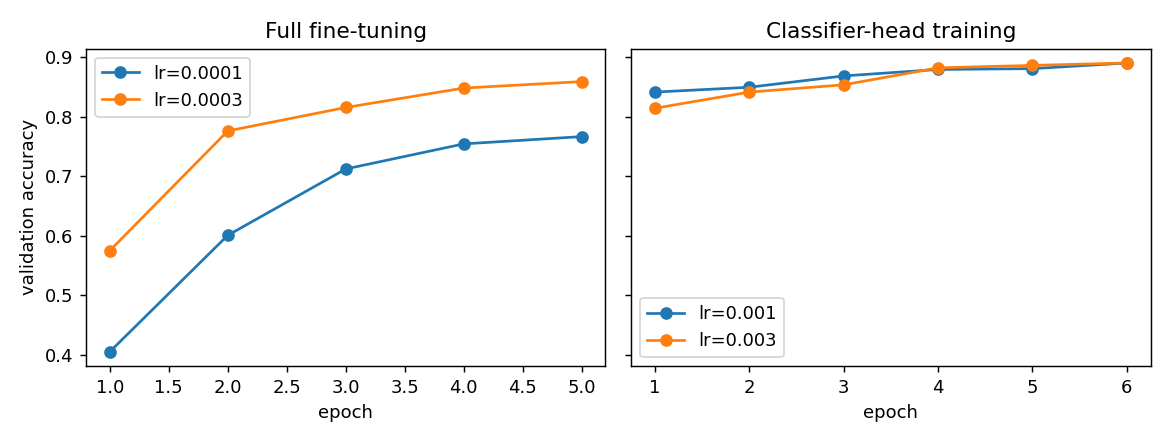
\includegraphics[width=0.78\linewidth]{validation_curves.png}
\caption{Validation accuracy per epoch for the candidate learning rates.}
\label{fig:curves}
\end{figure}

\textbf{Ranking.} Classifier-head training is best (86.9\% accuracy, 86.8\% macro-F1), followed by frozen features + logistic regression (85.7\%), linear SVM (83.3\%), random forest (82.7\%) and full fine-tuning (82.0\%).
Differences are small compared with the sampling uncertainty of a 3{,}669-image test set (95\% intervals of about $\pm1.1$--1.3 points): an exact McNemar test on the paired test predictions gives $p<10^{-18}$ for head vs.\ full fine-tuning and $p=0.002$ for head vs.\ logistic regression (132 vs.\ 86 images
correct for only one of them), but $p=0.22$ for full fine-tuning vs.\ random forest and $p=0.35$ for SVM vs.\ random forest, so those pairs are not distinguishable.
These tests only capture test-set sampling noise, not training randomness (single seed), so the $\approx1$-point head vs.\ logistic-regression difference should not be over-interpreted.

\textbf{Computational cost.} Frozen features are cheapest: one forward pass over the data (229\,s on this CPU) plus under 20\,s for the classifier, and a hyper-parameter grid costs seconds
once the features are cached. Head training still runs the frozen backbone forward at every epoch (augmentation prevents caching): 55--77\,s per epoch, versus 123--156\,s per epoch for full fine-tuning, which also back-propagates through all layers.
Full fine-tuning updates 2.5$\times$ more parameters than head training and was the slowest, yet it was not the most accurate.

\section{Errors}
\begin{figure}[h]
\centering
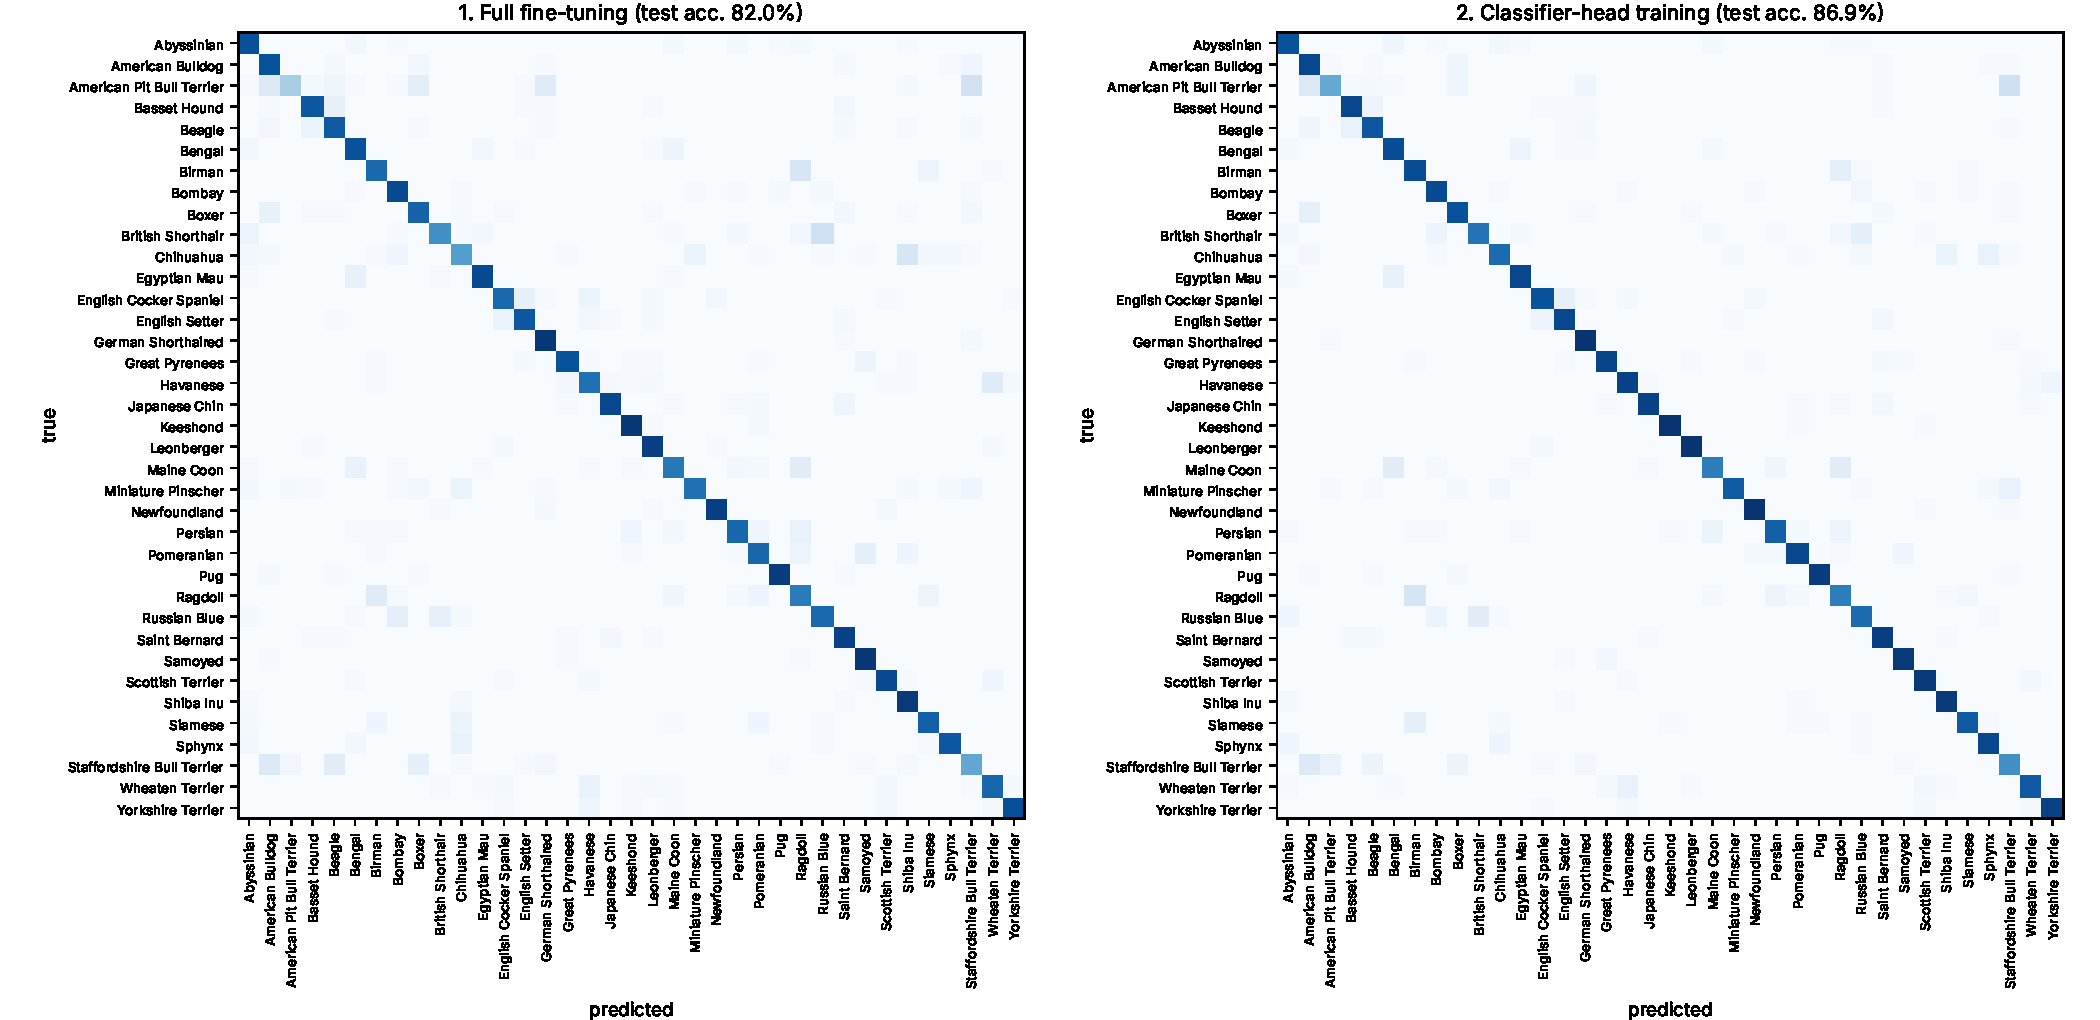
\includegraphics[width=\linewidth]{confusion_pair.pdf}
\caption{Row-normalised test confusion matrices with breed names (vector figure, zoom to read). Matrices of all approaches are in \texttt{results/figures/}.}
\label{fig:cm}
\end{figure}

\begin{figure}[h]
\centering
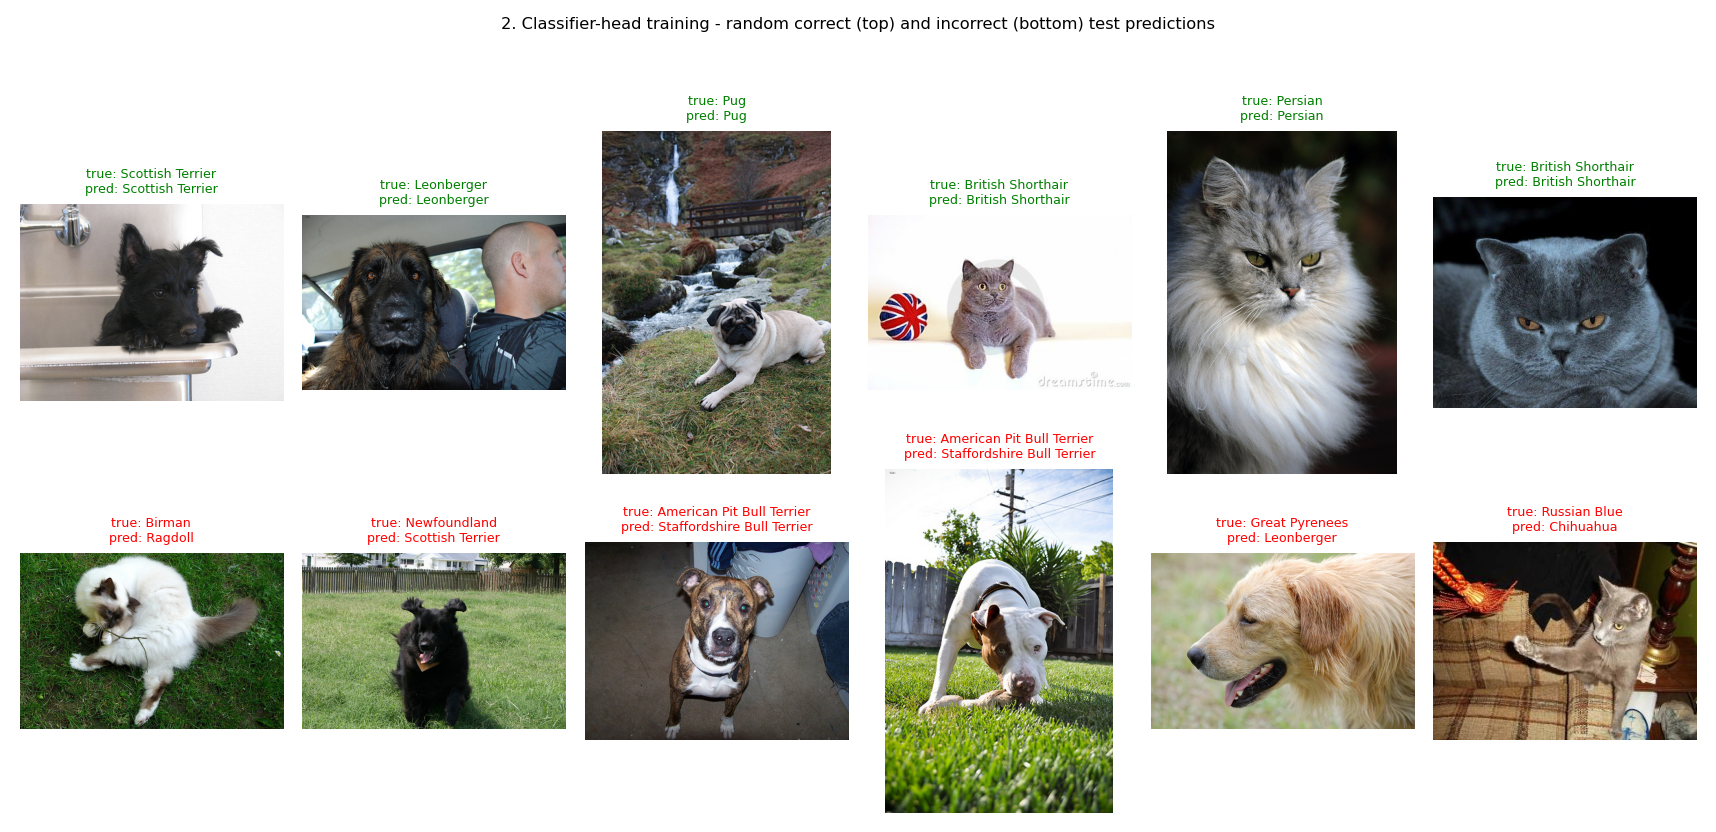
\includegraphics[width=\linewidth]{examples_head_training.png}
\caption{Random correct (top, green) and incorrect (bottom, red) test predictions of the best model (classifier-head training).}
\label{fig:ex}
\end{figure}

\begin{table}[h]
\centering\small
\begin{tabular}{llrrr}
\toprule
True breed & Predicted as & Head & Full FT & Log. reg. \\
\midrule
American Pit Bull Terrier & Staffordshire Bull Terrier & 21 & 19 & 18 \\
American Pit Bull Terrier & American Bulldog & 14 & 13 & 14 \\
Ragdoll & Birman & 17 & 12 & 15 \\
Birman & Ragdoll & 9 & 16 & 15 \\
British Shorthair & Russian Blue & 9 & 20 & 8 \\
Russian Blue & British Shorthair & 11 & 8 & 10 \\
Chihuahua & Shiba Inu & 6 & 16 & 10 \\
Maine Coon & Bengal & 11 & 7 & 12 \\
\bottomrule
\end{tabular}
\caption{Most frequent confusions (number of test images; each breed has 88--100).}
\label{tab:conf}
\end{table}

For the best model, 8 of 37 breeds reach at least 95\% recall, while the lowest recalls are American Pit Bull Terrier (52\%), Staffordshire Bull Terrier (63\%), Ragdoll (70\%), Maine Coon (70\%) and British Shorthair (74\%).
The mistakes are fine-grained and symmetric (Table~\ref{tab:conf}): American Pit Bull Terrier $\leftrightarrow$ Staffordshire Bull Terrier / American Bulldog, Ragdoll $\leftrightarrow$ Birman, British Shorthair $\leftrightarrow$ Russian Blue,
Chihuahua $\to$ Shiba Inu. About 85--89\% of all errors of every approach stay inside the same species (cat$\leftrightarrow$cat or dog$\leftrightarrow$dog; head training: 427 of 479 errors),
i.e.\ the features separate cats from dogs well and the difficulty is the within-species breed distinction, often with similar coat and body shape; the examples in Fig.~\ref{fig:ex} show typical cases.
Full fine-tuning is worst on the same breeds (American Pit Bull Terrier recall 34\%) and makes some confusions much more often (British Shorthair $\to$ Russian Blue: 20 vs.\ 9; Chihuahua $\to$ Shiba Inu: 16 vs.\ 6).

\section{Discussion}
\textbf{Overfitting and the train--test gap.} All approaches fit the training split much better than the test set (Table~\ref{tab:res}, with the 2{,}944 training images only $\approx$80 per breed).
The gap is largest for the models that interpolate the training features, random forest (100.0\% vs.\ 82.7\%, gap 17.3) and linear SVM (99.9\% vs.\ 83.3\%), followed by logistic regression (13.1) and full fine-tuning (13.0), and smallest for head training (10.3).
A plausible reason for the smaller gap of the two neural approaches is that they see augmented images and are stopped by validation accuracy, whereas the scikit-learn classifiers are fitted to a fixed set of 576-d vectors; I did not run an ablation to isolate this.
Full fine-tuning is not an overfitting case in the usual sense: its training loss (0.30) and validation accuracy were still improving at the last epoch (Fig.~\ref{fig:curves}) and the best epoch was the last for both learning rates. The result
mainly says that \emph{with 5 epochs on a CPU} it is not yet converged; the low-learning-rate run ($10^{-4}$) is clearly under-trained (76.6\% validation). Whether more epochs or a lower-then-higher learning rate for the backbone would let it overtake head training was not tested, so I do not claim that full fine-tuning is worse in general.
One hypothesis, not tested here, is that the freshly initialised 37-way layer produces large gradients that perturb the pre-trained features at the beginning of training.
For every approach the validation accuracy is about 2--4 points higher than the test accuracy; with only 736 validation images (standard error $\approx1.2$ points) and selection on it, this is expected.

\textbf{Dataset size and domain similarity.} The target domain is very close to the pre-training domain: ImageNet-1K contains about 120 dog-breed classes and several cat classes, so the frozen features are already highly discriminative for pets. This explains why training only a head, or even a linear classifier on frozen features,
reaches 86--87\% with 80 images per breed and little compute, and why updating the convolutional layers brings no benefit in our short budget. With such a small training set, adapting 1.5\,M parameters has more risk of drifting away from useful features than adapting 0.6\,M in the head; on a dataset further from ImageNet the balance would probably change.

\textbf{Trade-offs.} Frozen features + logistic regression give the best accuracy for their cost (85.7\% in about 230\,s, essentially all spent on feature extraction) and make tuning cheap. Head training gains about 1.2 points at 1.8$\times$ the time and stores a small model.
Full fine-tuning is the most flexible but the most expensive and, under our budget, the least accurate of the neural approaches.

\textbf{Limitations.} (i) One training run per approach and no seed-to-seed variance; (ii) only two learning rates per neural approach and few epochs, with the best epoch at the last one, and selected values at the edge of the grids for logistic regression ($C=0.01$) and random forest (300 trees), so better settings may exist; (iii) timings come from one CPU laptop and include data loading, so they are only comparable within this report; (iv) the validation set is small; (v) the McNemar tests ignore training randomness; (vi) the breed labels were not checked for noise or ambiguity.

\begin{thebibliography}{9}\small
\bibitem{parkhi2012} O.~M.~Parkhi, A.~Vedaldi, A.~Zisserman, C.~V.~Jawahar. Cats and dogs. \emph{CVPR}, 2012.
\bibitem{howard2019} A.~Howard et al. Searching for MobileNetV3. \emph{ICCV}, 2019.
\bibitem{paszke2019} A.~Paszke et al. PyTorch: An imperative style, high-performance deep learning library. \emph{NeurIPS}, 2019.
\bibitem{pedregosa2011} F.~Pedregosa et al. Scikit-learn: Machine learning in Python. \emph{JMLR} 12, 2011.
\end{thebibliography}
\end{document}
